\section{Introduction}
\begin{figure}  
	% \advance\leftskip-1cm 
	% \hspace*{0.25cm} 
	\centering
	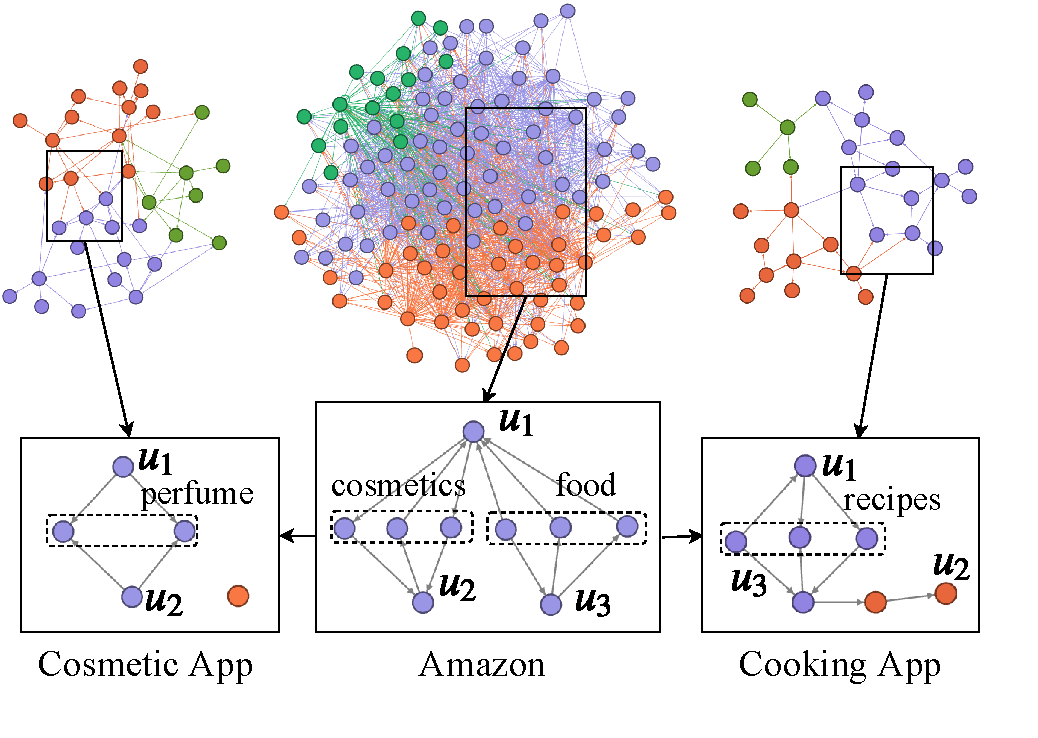
\includegraphics[width=0.8\columnwidth]{img/chapter4/example.pdf}
	%  \vspace{-1em}
	\caption{The Amazon graph is a main shopping graph while the Cosmetic App and the Cooking App are two small sparse graphs. Those graphs share mutual users in which three of them are selected to demonstrate their behaviors. Node colors indicate their related communities. }
	\label{fig:c4_example}
	%   \vspace{-1em}
\end{figure}

Community detection is an essential task for cyberspace mining, which has been successfully employed to explore users’ resemblance for retrieval/recommendation enhancement and user behavior analysis. Taking social media and e-commerce as examples, the complex, and often heterogeneous, relations among users and other objects, e.g., products, reviews, and messages, can be encapsulated as bipartite graphs, and the topology can help to synthesize and represent users with a coarser and broader view.

While a graph is well-connected, conventional methods, e.g., modularity-based approach \cite{newman2004fast}, spectral approach \cite{nascimento2011spectral}, dynamic approach \cite{peixoto2017modelling} and deep learning approach \cite{chiang2019cluster}, are able to estimate the internal/external connectivity and generate high-quality communities directly on nodes \cite{fortunato2016community}.

For a vulnerable graph with sparse connectivity, however, prior community detection algorithms can hardly probe enough information to optimize the community structure. Unfortunately, in the real cyberspace this can be a very common problem, i.e., while a handful of giant players (like Google, Facebook and Amazon) maintaining high-quality graphs, thousands of apps are suffering from graph cold start problem. If many users are isolated because of data sparseness, I can hardly tell any community information. 

In order to cope with this challenge, in this paper, I propose a novel research problem – Cross Graph Community Detection. The idea is based on the fact that an increasing number of small apps are utilizing the user identity information inherited from giant providers, i.e., users can easily login a large number of new apps by using Facebook and Google ID. In such ecosystem, the main large graph can provide critical information to enlighten the community detection on many small sparse graphs. Figure \ref{fig:c4_example} depicts an example, where the Cooking or Cosmetic Apps inherits important topological information from the main Amazon graph for their enhanced community detection. 

Note that, while the small sparse graphs can engage with a local field (like cooking or cosmetic in the example), the main graph can be quite comprehensive and noisy. As Figure \ref{fig:c4_example} shows, not all the connections in Amazon (shopping graph) can be equally important for the two candidate app graphs. Three mutual users are selected where $u_1$ and $u_2$ mainly share similar shopping interests on cosmetics and $u_1$ and $u_3$ mainly share similar shopping interests on food products in Amazon. Then, with deliberate propagation from main graph, in the Cosmetic graph, $u_1$ and $u_2$ have a better chance to be grouped together, while $u_1$ and $u_3$ are more likely to be assigned the same community ID in the Cooking graph. Therefore, the proposed model should be able to differentiate various kinds of information from the main graph for each candidate sparse graph to enhance its local community detection performance. 

As another challenge, small sparse graphs often suffer from training data insufficiency, e.g., the limited connections in these graphs can hardly tell the community residency information. In this study, I employed a novel data augmentation approach - cross graph pairwise learning. Given a candidate user and an associated user triplet, the proposed model can detection the community closeness superiority by leveraging main graph and the sparse graph simultaneously. Moreover, the proposed pairwise learning method can cope with the main graph heterogeneity issue and reduce noisy information by taking care of graph local structure. Theoretically, I can offer at most $\mathcal{O}(N^{3})$ user triplets to learn graph community structure while conventional community detection methods by default can only be applied on $\mathcal{O}(N)$ users  ($N$ is the number of users in the sparse graph).

Inspired by aforementioned discussion, I propose an innovative \textit{Pairwise Cross-graph Community Detection} (PCCD) model for enhanced sparse graph user community detection. Specifically, given user $u_i$ and its associated triplet $\langle u_{i},u_{j},u_{k}\rangle$, I aim to predict their pairwise community relationship, e.g., compared with user $u_{k}$, user $u_{j}$ should have closer, similar or farther community closeness to user $u_i$. The contribution of this paper is fourfold: 
\begin{itemize}
	\item I propose a novel problem - Cross Graph Community Detection, which can be critical for thousands of small businesses or services if they enable external user account login.
	
	\item Unlike conventional community detection methods, I explore community structure from a pairwise viewpoint. In this way, I can efficiently deal with graph heterogeneous information and solve cold-start problem for users with no behaviors in sparse graphs.
	
	\item The proposed model is trained in an end-to-end manner where a two-level filtering module locates the most relevant information to propagate between graphs. A Community Recurrent Unit (CRU) subsequently learns user community distribution from the filtered information.
	
	\item Extensive experiments on two real-world cross-graph datasets validate my model superiority. I also evaluate my model robustness on graphs with varied sparsity scales and many other supplementary studies.  
\end{itemize} 

